\documentclass[journal]{IEEEtran}
\usepackage{cite}
\usepackage{amsmath,amssymb,amsfonts}
\usepackage{graphicx}
\usepackage{textcomp}
\usepackage{xcolor}
\usepackage{booktabs}
\usepackage{url}
\usepackage{hyperref}
\usepackage{tabularx}
\usepackage{multirow}
\usepackage{fontspec}
\usepackage{kotex}

\begin{document}

\title{KOSHA-Braille: Infrastructure-Grade Accessibility for Korean Chemical Safety Information}

\author{Yu~Yong~Kim
\thanks{Manuscript submitted April 2026.}
\thanks{Y.~Y.~Kim is with the University of Wisconsin--Madison, Madison, WI 53706, USA (e-mail: ykim288@wisc.edu).}
}

\markboth{IEEE Access, VOL. XX, NO. X, 2026}
{Kim: KOSHA-Braille}

\begin{abstract}
Accessibility to high-stakes technical information---chemical safety, legal statutes, medical documentation---is a prerequisite for participation in the professions that govern them. For visually impaired readers, such participation presumes the existence of braille infrastructure for those domains. For Korean chemical safety, no such infrastructure has existed, producing a self-fulfilling exclusion: without braille access to Material Safety Data Sheets (MSDS), visually impaired individuals cannot readily enter chemistry-adjacent roles in research, regulation, labor advocacy, or public office; absent such participants, the case for producing the infrastructure is never made. This paper presents KOSHA-Braille, a deliberate attempt to break that cycle by providing infrastructure ahead of demonstrated demand. We construct a large-scale Korean chemical safety braille corpus of 48,966 chemicals and 769,897 MSDS sections (232.3 million braille cells) using a deterministic encoder compliant with the 2017 Korean Braille Standards, cross-validated with an independent open-source implementation at 100\% agreement over 442 test cases. The dataset, encoder, and a reference web service are released publicly. We argue that the appropriate measure of such work is not adoption volume but parity of access under the UN Convention on the Rights of Persons with Disabilities (Article~9) and Korea's Anti-Discrimination Against Persons with Disabilities Act (Article~21). The underlying architecture is domain- and language-extensible and provides a template for analogous accessibility infrastructure in adjacent high-stakes domains.
\end{abstract}

\begin{keywords}
Accessibility infrastructure, braille, chemical safety, MSDS, Korean braille, visually impaired, GHS, occupational health, disability rights, dataset.
\end{keywords}

\titlepgskip=-15pt

\maketitle

\section{Introduction}
\label{sec:introduction}

\subsection{Accessibility as Infrastructure, Not Service}

Public accessibility systems---tactile paving, screen-door platforms, audio description on broadcast media, sign-language interpretation of parliamentary proceedings---share a structural property: their legitimacy is not contingent on per-day usage counts. They are infrastructure. Their function is to establish the conditions under which participation by persons with disabilities becomes possible at all. Evaluating such systems by market-style demand metrics conflates \emph{service} (discretionary, elastic) with \emph{infrastructure} (foundational, inelastic) and systematically undervalues low-incidence, high-stakes access.

This paper applies that lens to a domain where the gap is particularly stark: chemical safety information in the Korean regulatory regime. Material Safety Data Sheets (MSDS), internationally known as Safety Data Sheets (SDS), are mandatory documents containing hazard classifications, safe handling procedures, emergency measures, and exposure-limit information \cite{kosha_act}. They are read by chemists, industrial hygienists, emergency responders, occupational safety inspectors, injured-worker attorneys, journalists, legislators, and trade-union organizers. In South Korea these documents are produced exclusively as visual text under the Occupational Safety and Health Act \cite{kosha_act}, rendering them inaccessible to braille readers.

\subsection{The Self-Fulfilling Exclusion Problem}

The most common objection to producing domain-specific braille infrastructure is that the expected user population is small. In Korean chemical safety specifically, the observable population of visually impaired chemists, chemical engineers, or chemical-safety regulators is close to zero. We argue this observation is not evidence against infrastructure but evidence \emph{for} it: low observable participation in a profession is a predictable consequence of inaccessible professional information, not an independent fact about preference or capability.

Precedents for visually impaired participation in chemistry-adjacent work exist where infrastructure has been built or improvised: Henry ``Hoby'' Wedler, who completed a PhD in computational organic chemistry at the University of California, Davis in 2016 with the support of a 3D-printed molecular-model accessibility apparatus and subsequently founded Accessible Science to extend chemistry instruction to visually impaired students \cite{wedler}; blind legislators handling technical portfolios in multiple jurisdictions \cite{nfb_legislators}; disability-rights organizations conducting chemical-exposure litigation and regulatory advocacy. These cases demonstrate that the capability and interest are present; what is absent in the Korean case is the reading infrastructure.

The situation is further shaped by secondary readers who are not themselves chemists but must read MSDS professionally: legislative staff preparing questions for a minister of trade and industry, labor inspectors documenting an industrial accident, attorneys litigating occupational-disease claims, journalists investigating chemical-plant incidents, and civil-society organizers mobilizing around semiconductor-sector injuries. Each of these roles is a potential site of visually impaired participation, and each is foreclosed---silently---by the absence of braille MSDS infrastructure.

\subsection{Legal and Normative Basis}

Two instruments frame the obligation:

\begin{enumerate}
\item \textbf{UN Convention on the Rights of Persons with Disabilities, Article~9 (Accessibility)} \cite{crpd}: State parties shall take appropriate measures to ensure that persons with disabilities have access, on an equal basis with others, to information and communications, including information and communications technologies and systems. South Korea ratified the CRPD in 2008.

\item \textbf{Act on the Prohibition of Discrimination Against Persons with Disabilities, Article~21} \cite{kdpa}: Requires accessible-format provision of public-interest information. Chemical safety information produced by a public agency (KOSHA) under a statutory mandate falls within this scope.
\end{enumerate}

The absence of a chemical-safety braille service is therefore not a neutral market outcome; it is non-performance of an existing obligation. The question addressed by this paper is not whether such infrastructure should exist, but how to construct it at sufficient scale, fidelity, and extensibility to constitute infrastructure rather than demonstration.

\subsection{Contributions}

\begin{enumerate}
\item \textbf{Framing contribution}: We articulate chemical safety information as an infrastructure-grade accessibility target and establish the evaluation criteria appropriate to that framing: parity of coverage, standards compliance, determinism, and extensibility, rather than adoption volume.

\item \textbf{KOSHA-Braille corpus}: A public Korean chemical safety braille corpus of 48,966 chemicals and 769,897 MSDS sections---approximately 119.3 million Korean characters and 232.3 million braille cells. To our knowledge, the largest Korean-language braille corpus of any kind released to date, and the first for any chemical-safety regime in any language.

\item \textbf{Standards-compliant deterministic encoder}: A rule-based Korean braille encoder implementing the 2017 Korean Braille Standards, cross-validated at 100\% agreement over 442 test cases against an independent open-source implementation.

\item \textbf{Mixed-script handling for technical content}: Rule-consistent braille indicator handling (Roman letter indicator, number indicator, capital indicator) for the Korean--Latin--numeric script mixture characteristic of MSDS; GHS pictogram codes resolved to descriptive Korean text for semantic rather than visual reference.

\item \textbf{Reference deployment}: A freely accessible web service providing search, real-time conversion, and file downloads in embosser-ready BRF and refreshable-display Unicode formats.

\item \textbf{Extensibility analysis} (Section~\ref{sec:extensibility}): Explicit treatment of the architectural properties that make the system a template for adjacent high-stakes accessibility domains (pharmaceutical labels, food allergens, first-aid protocols, chemical registration filings) and for adaptation across languages and regulatory regimes.
\end{enumerate}

\section{Related Work}
\label{sec:related}

\subsection{Accessibility Infrastructure}

Policy and design literature distinguish \emph{assistive services}, which respond to individual requests, from \emph{accessibility infrastructure}, which pre-installs the conditions for access. Hamraie's history of universal design \cite{hamraie} documents how accessibility provisions originated as targeted disability interventions but were progressively recognized as foundational built-environment features. Blackwell's articulation of the ``curb-cut effect'' \cite{curb_cut} generalizes the pattern: design changes initially intended for an underserved group consistently yield broader benefits, but only after the original intervention has been built ahead of demonstrated demand. Bennett and Keyes \cite{bennett_keyes} further argue that disability-related technical interventions framed in terms of marginal ``fairness'' calculations systematically miss the structural-justice dimension; the appropriate frame is whether the structural conditions for participation exist at all.

The present work positions domain-specific braille corpora for technical and regulatory information as a category of accessibility infrastructure that has been systematically underproduced, particularly outside English. Standard examples---captioning systems, public-library braille collections, audio description, sign-language interpretation of legislative proceedings---are characteristically produced in advance of measured demand and justified by rights frameworks rather than marginal-utility calculations.

\subsection{Braille Translation Systems}

Braille translation is most extensively studied for English via liblouis \cite{liblouis}, an open-source translator supporting more than 100 languages. For Korean, liblouis provides Grade~1 and Grade~2 tables based on the 2006 standards; a small number of open-source projects implement the 2017 revisions \cite{hangul_braille_converter,hanbraille}. These tools are character-level translators and do not address domain-level concerns such as consistent handling of regulatory codes, scientific notation within safety text, or large-scale corpus construction.

\subsection{Chemical Safety Information Accessibility}

The Globally Harmonized System (GHS) \cite{ghs} standardizes visual hazard communication but specifies no braille counterpart. The European Union mandates braille on pharmaceutical packaging \cite{eu_braille}, the narrowest precedent for regulated braille in chemistry-adjacent domains; this applies to product names only, not to safety documentation. We are not aware of prior work on braille SDS/MSDS in any language.

\subsection{Korean Braille Standards}

The 2017 Korean Braille Standards \cite{ko_braille_2017} were promulgated by the Ministry of Culture, Sports and Tourism. Korean braille is syllable-structured: each Hangul block decomposes into initial consonant, vowel, and optional final consonant, with each component mapped to a fixed dot pattern. The 2017 revision expanded coverage to six domains including scientific notation and music notation.

\section{System Architecture}
\label{sec:system}

\subsection{Data Pipeline}

The system comprises four stages, illustrated in Fig.~\ref{fig:pipeline}: acquisition, extraction, encoding, and delivery.

\begin{figure*}[t]
\centering

\includegraphics[width=\textwidth]{fig_pipeline.pdf}
\caption{System architecture of KOSHA-Braille. MSDS data is acquired from the KOSHA public API, parsed and cleaned (including GHS pictogram conversion), encoded to Korean braille following the 2017 standards, and served through a web interface.}
\label{fig:pipeline}
\end{figure*}

\begin{enumerate}
\item \textbf{Data Acquisition}: KOSHA MSDS data is retrieved via the Korea Public Data Portal REST API \cite{data_go_kr}, providing 16 standardized MSDS sections per chemical in XML format.

\item \textbf{Text Extraction}: XML responses are parsed for Korean text content. GHS pictogram references (e.g., ``GHS06.gif'') are resolved to descriptive Korean text (e.g., ``{급성독성}'') so that braille output conveys semantic hazard information rather than an unreadable filename.

\item \textbf{Braille Encoding}: Korean text is converted to Unicode braille (U+2800--U+28FF) following the 2017 Korean Braille Standards.

\item \textbf{Delivery}: A FastAPI backend serves the encoded content through a REST API; the reference single-page frontend provides search and side-by-side visual/braille viewing; downloads are offered in embosser-format BRF and Unicode \texttt{.txt}.
\end{enumerate}

\subsection{Korean Braille Encoding}

The encoding process is deterministic and lossless. Each Hangul syllable is decomposed using Unicode arithmetic into initial consonant, vowel, and final consonant, each mapping to a fixed dot pattern.

The encoder handles four character types with appropriate braille indicators:

\begin{itemize}
\item \textbf{Hangul}: direct decomposition to braille dot patterns (no indicator needed).
\item \textbf{Numbers}: number indicator (dots 3-4-5-6) followed by digit patterns.
\item \textbf{Latin letters}: Roman letter indicator (dots 3-5-6) followed by letter patterns; uppercase adds capital indicator (dot 6).
\item \textbf{Punctuation}: direct mapping to Korean braille punctuation patterns.
\end{itemize}

Double consonants use a dot-6 prefix cell followed by the base consonant pattern. Compound vowels and compound final consonants use multi-cell sequences.

Tables~\ref{tab:cho}, \ref{tab:jung}, and \ref{tab:jong} show the complete mapping for initial consonants, vowels, and final consonants, respectively.

\begin{table}[h]
\centering
\caption{Initial Consonant Braille Patterns}
\label{tab:cho}
\begin{tabular}{cccc}
\toprule
Consonant & Dots & Consonant & Dots \\
\midrule
{ㄱ} & 4 & {ㅅ} & 6 \\
{ㄴ} & 1-4 & {ㅇ} & 1-2-4-5 \\
{ㄷ} & 2-4 & {ㅈ} & 4-6 \\
{ㄹ} & 5 & {ㅊ} & 5-6 \\
{ㅁ} & 1-5 & {ㅋ} & 1-2-4 \\
{ㅂ} & 4-5 & {ㅌ} & 1-2-5 \\
& & {ㅍ} & 1-4-5 \\
& & {ㅎ} & 2-4-5 \\
\bottomrule
\end{tabular}
\end{table}

\begin{table}[h]
\centering
\caption{Vowel Braille Patterns}
\label{tab:jung}
\begin{tabular}{cccc}
\toprule
Vowel & Dots & Vowel & Dots \\
\midrule
{ㅏ} & 1-2-6 & {ㅗ} & 1-3-6 \\
{ㅐ} & 1-2-3-5 & {ㅛ} & 3-4-6 \\
{ㅑ} & 3-4-5 & {ㅜ} & 1-3-4 \\
{ㅓ} & 2-3-4 & {ㅠ} & 1-4-6 \\
{ㅔ} & 1-3-4-5 & {ㅡ} & 2-4-6 \\
{ㅕ} & 1-5-6 & {ㅢ} & 2-4-5-6 \\
{ㅖ} & 3-4 & {ㅣ} & 1-3-5 \\
\bottomrule
\end{tabular}
\end{table}

\begin{table}[h]
\centering
\caption{Final Consonant Braille Patterns}
\label{tab:jong}
\begin{tabular}{cccc}
\toprule
Consonant & Dots & Consonant & Dots \\
\midrule
{ㄱ} & 1 & {ㅇ} & 2-3-5-6 \\
{ㄴ} & 2-5 & {ㅈ} & 1-3 \\
{ㄷ} & 3-5 & {ㅊ} & 2-3 \\
{ㄹ} & 2 & {ㅋ} & 2-3-5 \\
{ㅁ} & 2-6 & {ㅌ} & 2-3-6 \\
{ㅂ} & 1-2 & {ㅍ} & 2-5-6 \\
{ㅅ} & 3 & {ㅎ} & 3-5-6 \\
\bottomrule
\end{tabular}
\end{table}

\section{Dataset Description}
\label{sec:dataset}

\subsection{Source Data}

The KOSHA-Braille dataset is derived from the Korea Occupational Safety and Health Agency (KOSHA) Material Safety Data Sheet database, accessed through the Korea Public Data Portal API \cite{data_go_kr} under an authorized operational account with a daily limit of 100,000 calls per endpoint.

\subsection{Dataset Statistics}

Table~\ref{tab:stats} summarizes the dataset characteristics. Fig.~\ref{fig:stats} shows the character distribution and text-length distribution.

\begin{figure}[t]
\centering

\includegraphics[width=\columnwidth]{fig_dataset_stats.pdf}
\caption{Dataset characteristics. (Left) Character type distribution across all MSDS text. (Right) Distribution of total text length per chemical substance.}
\label{fig:stats}
\end{figure}

\begin{table}[h]
\centering
\caption{KOSHA-Braille Dataset Statistics}
\label{tab:stats}
\begin{tabular}{lr}
\toprule
Metric & Value \\
\midrule
Total chemicals & 48,966 \\
MSDS sections per chemical & 15--16 \\
Total sections & 769,897 \\
Korean text (total) & 119.3 M chars \\
Korean braille (total) & 232.3 M cells \\
Avg.\ Korean text per chemical & 6,046 chars \\
Median text per chemical & 5,934 chars \\
Std.\ deviation & 1,435 chars \\
Min / Max text & 2,241 / 10,490 chars \\
Mean braille:text ratio & 1.95 \\
\midrule
Korean characters & 76.3\% \\
Latin characters & 16.6\% \\
Numeric characters & 7.1\% \\
\bottomrule
\end{tabular}
\end{table}

\subsection{GHS Pictogram Conversion}

Original MSDS data references GHS hazard pictograms as image filenames (e.g., ``GHS06.gif''), which are meaningless in braille. The system resolves these to descriptive Korean text as shown in Table~\ref{tab:ghs}. All 147 unique H/P statement codes occurring in the database (63 H-statements, 84 P-statements) are resolved and encoded.

\begin{table}[h]
\centering
\caption{GHS Pictogram to Korean Text Conversion}
\label{tab:ghs}
\begin{tabular}{lll}
\toprule
Code & English & Korean \\
\midrule
GHS01 & Explosive & {폭발성} \\
GHS02 & Flammable & {인화성} \\
GHS03 & Oxidizing & {산화성} \\
GHS04 & Compressed gas & {고압가스} \\
GHS05 & Corrosive & {부식성} \\
GHS06 & Acute toxicity & {급성독성} \\
GHS07 & Irritant & {경고} \\
GHS08 & Health hazard & {건강유해성} \\
GHS09 & Environmental & {수생환경유해성} \\
\bottomrule
\end{tabular}
\end{table}

\subsection{Release}

The full corpus is released as a single JSONL file (943~MB) in HuggingFace-compatible schema, with a dataset card specifying provenance, license, section schema, and intended use. The encoder, decoder, and reference service are released as open-source code.

\section{Validation}
\label{sec:validation}

\subsection{Deterministic Correctness}

Korean braille encoding under the 2017 standards is a deterministic, rule-defined transformation. Each Hangul syllable decomposes unambiguously into initial, medial, and optional final, each mapping to a fixed dot pattern. Correctness therefore reduces to verifying the mapping tables and their application, rather than requiring per-output human-transcriber evaluation---an important property for infrastructure-scale corpora where sample-based human validation cannot reach global coverage.

\subsection{Cross-Reference Validation}

The encoder was validated against an independently developed open-source Korean braille converter \cite{hangul_braille_converter}. Table~\ref{tab:validation} shows the results.

\begin{table}[h]
\centering
\caption{Cross-Reference Validation Results}
\label{tab:validation}
\begin{tabular}{lrr}
\toprule
Test Set & Samples & Agreement \\
\midrule
Basic Hangul syllables & 41 & 100\% \\
Korean golden sentences & 45 & 100\% \\
MSDS chemical names & 356 & 100\% \\
\midrule
\textbf{Total} & \textbf{442} & \textbf{100\%} \\
\bottomrule
\end{tabular}
\end{table}

\subsection{Encoding Properties}

\begin{itemize}
\item \textbf{Deterministic}: identical input always produces identical output.
\item \textbf{Injective}: verified zero collisions across 37 distinct syllables.
\item \textbf{Standards-compliant}: all dot patterns match the 2017 Korean Braille Standards \cite{ko_braille_2017}.
\end{itemize}

\subsection{Scope of Validation}

This validation establishes correctness of the encoding mapping against a reference implementation and the published standard. It does not include a reading-comprehension user study with visually impaired readers, which we identify as essential follow-up work. Grade~2 contracted Korean braille is not implemented; the corpus is Grade~1 throughout.

\section{Reference Deployment}
\label{sec:webservice}

\subsection{Architecture}

The web service is built on FastAPI (Python) with a single-page HTML/JavaScript frontend. SQLite stores pre-fetched MSDS XML; braille conversion is on-demand with typical response times under 500\,ms per chemical.

\subsection{API Endpoints}

\begin{itemize}
\item \texttt{GET /api/stats} -- corpus statistics
\item \texttt{GET /api/chemicals?search=} -- search by Korean name or CAS number
\item \texttt{GET /api/chemicals/\{id\}} -- full MSDS text
\item \texttt{GET /api/chemicals/\{id\}/braille} -- MSDS with Korean braille
\item \texttt{GET /api/chemicals/\{id\}/braille.txt} -- Unicode braille download
\item \texttt{GET /api/chemicals/\{id\}/braille.brf} -- BRF (embosser) download
\item \texttt{POST /api/convert} -- ad-hoc Korean$\rightarrow$braille
\end{itemize}

\subsection{User Interface and Consumption Paths}

The visual side-by-side view (Fig.~\ref{fig:webui}) is a presentation surface for sighted stakeholders (regulators, procurement officers, auditors) who must verify that braille production exists and is consistent with the Korean source. The functionally important outputs for braille readers are the downloadable BRF and Unicode files, which feed directly into: (1) refreshable braille displays over USB or Bluetooth from a local machine or phone; (2) braille embossers for hard-copy output; (3) accessible reading software on desktop and mobile. The deployment is explicitly a reference implementation, not a product; its purpose is to demonstrate that the corpus is consumable end-to-end with existing assistive hardware and software.

\begin{figure}[t]
\centering
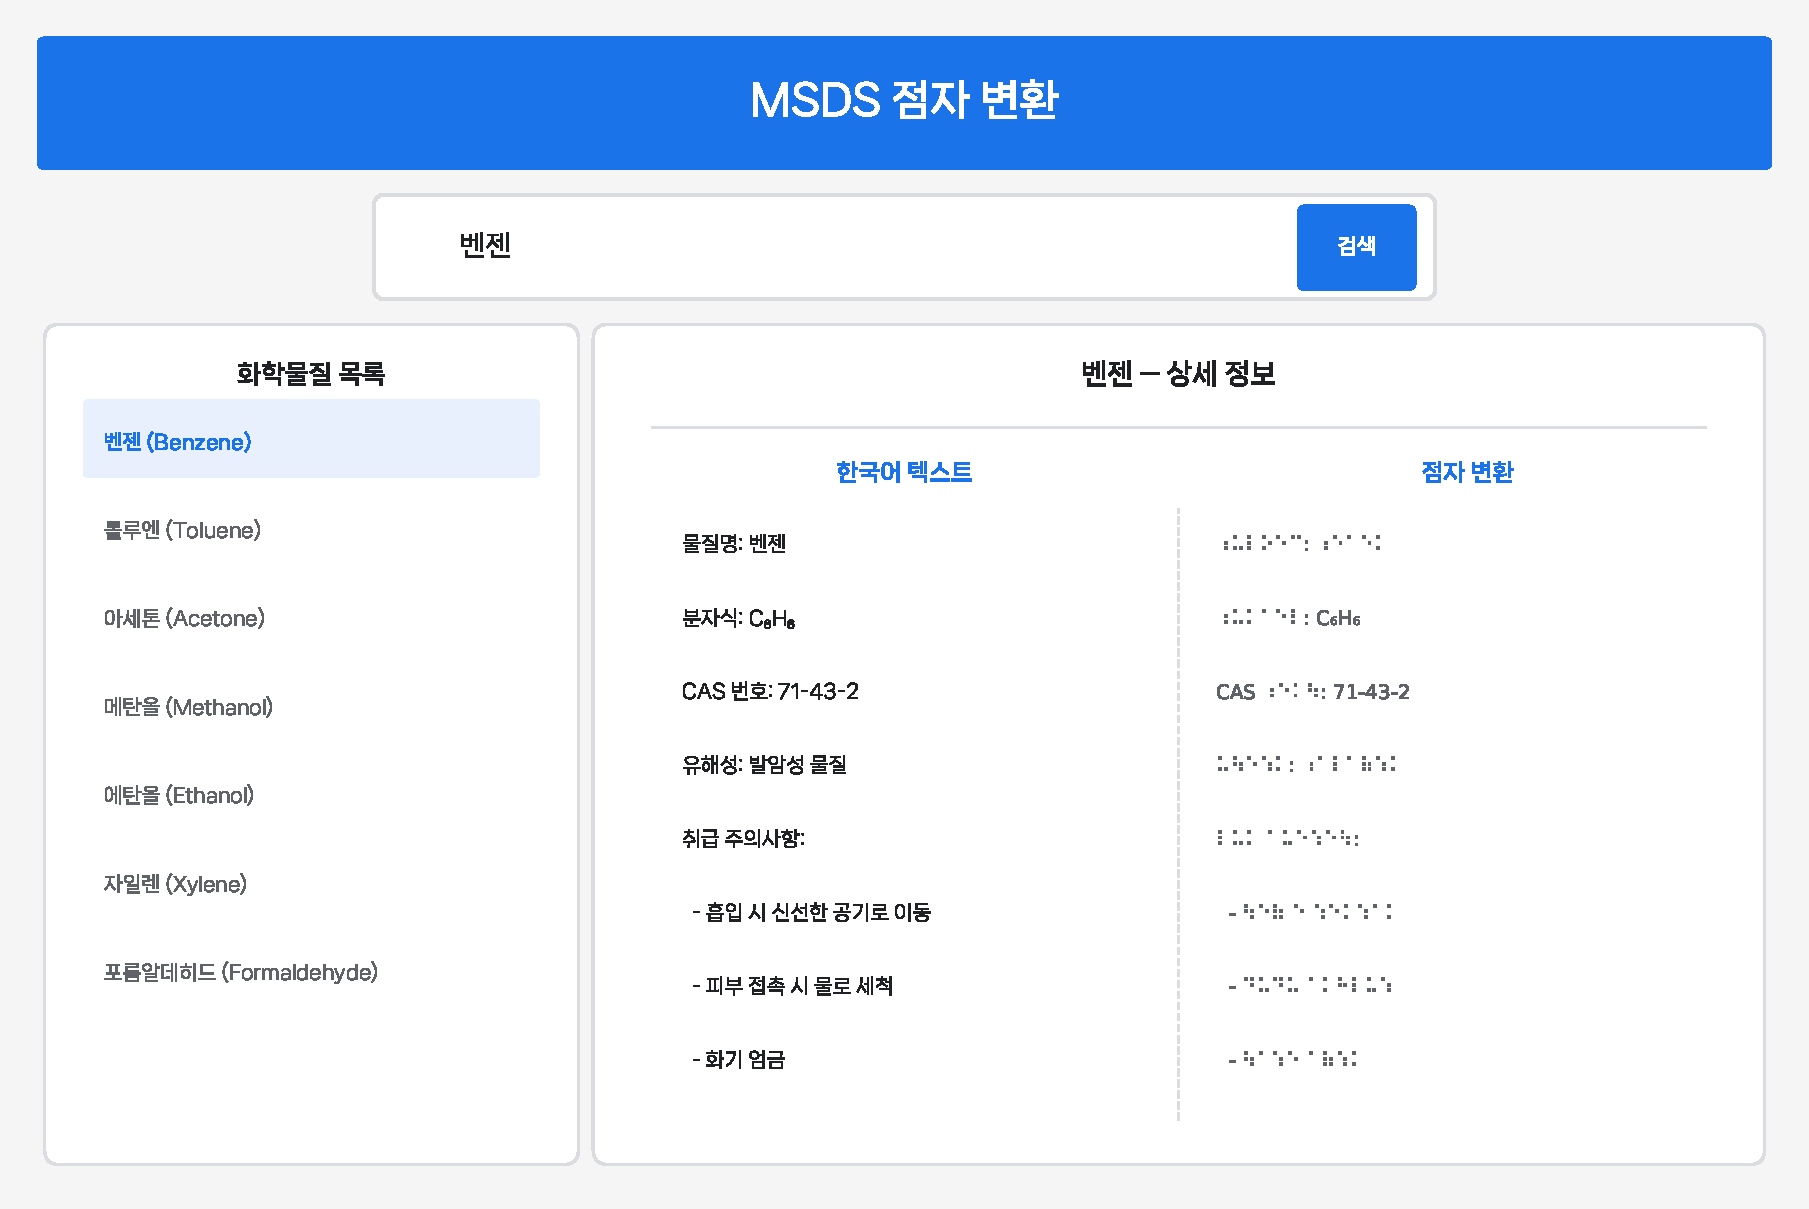
\includegraphics[width=\columnwidth]{fig_webui.pdf}
\caption{Web service user interface showing chemical search (top), result list (left), and side-by-side Korean text and braille display (right).}
\label{fig:webui}
\end{figure}

\section{Extensibility}
\label{sec:extensibility}

A central claim of this paper is that KOSHA-Braille is a template, not a terminus.

\subsection{Domain Extensibility}

The pipeline is structured around a structured regulatory source, an XML/JSON extractor, a language-specific deterministic braille encoder, and a delivery layer. Natural extensions include:

\begin{itemize}
\item \textbf{Pharmaceutical labels and inserts} (Korean Ministry of Food and Drug Safety): the narrowest existing international precedent for regulatory braille (EU pharmaceutical packaging \cite{eu_braille}) is product-name only; full-label braille is a direct extension.
\item \textbf{Food allergen statements}: 19 categories enumerated in Korean food-labeling regulation. A preliminary export is included in the current release.
\item \textbf{First-aid and occupational-health protocols}: KISCHEM first-aid records ($n=7{,}189$) exported in the current release.
\item \textbf{Chemical registration and disclosure filings} under Korean K-REACH (47,344 registered substances).
\item \textbf{Legal statutes and administrative rulings} concerning occupational safety and chemical regulation.
\end{itemize}

\subsection{Language Extensibility}

The only language-specific component is the encoder. Substitution of a rule table for another braille standard---Japanese (2001), Chinese (Mandarin Braille), English UEB, EU-country standards---preserves the remainder of the pipeline. Because GHS codes and CAS numbers are language-agnostic, cross-language interoperation is natural: 74,494 CAS numbers in KOSHA records provide a bridge to PubChem, ECHA, EPA, and OSHA registries.

\subsection{Regulatory-Regime Extensibility}

The ``structured regulatory source $\rightarrow$ braille corpus'' pattern applies to OSHA HazCom SDS (US), CLP/REACH SDS (EU), J-CHECK (Japan), and comparable national regimes. Adaptation requires only ingest code against the national data portal and substitution of the braille standard.

\subsection{Consumption-Format Extensibility}

The current release provides Unicode braille (U+2800--U+28FF) and BRF. Near-term extensions include Tactile SVG for embossed/thermoformed rendering, tactile-graphics derivatives of GHS pictograms, and JSON-LD annotations linking CAS and ICSC identifiers.

\subsection{Policy Extensibility}

The corpus is a concrete artifact against which policy proposals can be made: KOSHA adoption as an official accessible format; inclusion in Ministry-of-Employment-and-Labor procurement standards; integration into enterprise EHS systems with braille-embosser output.

\section{Discussion}
\label{sec:discussion}

\subsection{The Appropriate Evaluation Criterion}

We are explicit that KOSHA-Braille is not evaluated by adoption volume. The appropriate criteria for infrastructure-grade accessibility artifacts are:

\begin{enumerate}
\item Parity of coverage with the sighted-reader counterpart (here, 100\% of KOSHA MSDS records).
\item Standards compliance (verified in Section~\ref{sec:validation}).
\item Determinism and reproducibility.
\item Availability (freely accessible; no institutional or paywall gating).
\item Extensibility (Section~\ref{sec:extensibility}).
\end{enumerate}

By these criteria the present system is a substantial advance: prior state of the art for Korean chemical-safety braille was null.

\subsection{Low-Incidence High-Stakes Accessibility}

Chemical safety is one instance of a broader class of accessibility targets: technical and regulatory information domains with small observed visually impaired user populations but high consequences when access is absent. Other members of this class include legal statutes and case law, medical guidelines, standards documents, and public-administration reference materials. The economic objection to building braille infrastructure for these domains is identical in each case, and is rebutted identically: the observed user count is a function of the infrastructure, not an independent fact about it.

\subsection{Known Limitations}

\begin{enumerate}
\item \textbf{No reading-comprehension user study}: validated by determinism and reference-implementation cross-check, not by visually impaired reader evaluation.
\item \textbf{Grade~1 only}: Korean Grade~2 contractions would shorten documents but introduce context-dependent abbreviation decisions incompatible with strict determinism at this stage.
\item \textbf{Decoder ambiguity at the 초성/종성 boundary}: inherent to Korean braille; relevant to round-trip metrics only.
\item \textbf{Domain terminology in translated source}: machine-translated MSDS content (where used) may carry domain-term errors that propagate to braille.
\end{enumerate}

\section{Conclusion}
\label{sec:conclusion}

We have presented KOSHA-Braille as accessibility infrastructure for Korean chemical safety information: a 48,966-chemical, 769,897-section, 232.3-million-cell braille corpus produced by a deterministic, standards-compliant encoder and released publicly with a reference deployment. We argued that the appropriate framing for such work is infrastructure provision under Article~9 of the UN CRPD \cite{crpd} and Article~21 of Korea's Anti-Discrimination Against Persons with Disabilities Act \cite{kdpa}, not volume-driven service delivery. We identified and treated in Section~\ref{sec:extensibility} the architectural properties that make the system extensible across domains (pharmaceutical labels, food allergens, first-aid protocols, K-REACH filings, legal text), languages (by substitution of the braille encoder), and regulatory regimes (OSHA, CLP/REACH, J-CHECK).

The case for this kind of work should not rest on how many readers use it next month. It rests on who cannot enter a profession---whose question cannot be asked in a national assembly, whose claim cannot be pursued in court, whose investigation cannot be filed in a newsroom---when the necessary reading infrastructure does not exist. Future work includes reading-comprehension user studies with visually impaired readers, Grade~2 contracted-braille support, tactile-graphics treatment of GHS pictograms, and adoption by relevant regulators as an official accessible format.

\section*{Data Availability}

The dataset is released publicly on HuggingFace Datasets as \texttt{Yuyongkim/inconvenience-msds} \cite{hf_dataset} and the source code (encoder, decoder, pipeline, web service, evaluation harness) on GitHub at \texttt{yuyongkim/inconvenience-msds} \cite{github_repo}. The MSDS source data is publicly available through the Korea Public Data Portal \cite{data_go_kr}. Dataset license: CC BY 4.0; code license: MIT.

\begin{thebibliography}{20}

\bibitem{kosha_act}
Ministry of Employment and Labor, ``Occupational Safety and Health Act,'' Arts.~110--111, Republic of Korea, 2020.

\bibitem{crpd}
United Nations General Assembly, ``Convention on the Rights of Persons with Disabilities,'' Art.~9 (Accessibility), Resolution A/RES/61/106, adopted 13~December 2006, entered into force 3~May 2008.

\bibitem{kdpa}
Republic of Korea, ``Act on the Prohibition of Discrimination Against Persons with Disabilities and Remedy Against Infringement of Their Rights,'' Act No.~8341 (2007), latest amendment Act No.~10280; esp.\ Arts.~20--21 (Information Access). Official English translation: Korea Legal Research Institute, \url{https://elaw.klri.re.kr/}.

\bibitem{hamraie}
A.~Hamraie, \emph{Building Access: Universal Design and the Politics of Disability}. Minneapolis, MN: Univ.\ of Minnesota Press, 2017. ISBN 978-1-5179-0164-6.

\bibitem{curb_cut}
A.~G.~Blackwell, ``The curb-cut effect,'' \emph{Stanford Social Innovation Review}, vol.~15, no.~1, pp.~28--33, Winter 2017. DOI:~10.48558/YVMS-CC96.

\bibitem{bennett_keyes}
C.~L.~Bennett and O.~Keyes, ``What is the point of fairness? Disability, AI and the complexity of justice,'' \emph{ACM SIGACCESS Accessibility and Computing}, no.~125, art.~1, Mar.~2020. DOI:~10.1145/3386296.3386301.

\bibitem{wedler}
University of California, Davis, ``White House hails blind chemistry grad student as `Champion of Change','' UC~Davis News, July~2012; H.~Wedler, Ph.D.\ dissertation, Dept.\ of Chemistry, Univ.\ of California, Davis, 2016; Accessible Science, \url{https://accessiblescience.com/}.

\bibitem{nfb_legislators}
National Federation of the Blind, ``Blind Legislators and Public Officials,'' \url{https://nfb.org/}, accessed 2026.

\bibitem{disability_stats}
Korea Disabled People's Development Institute, ``2023 Disability Statistics Annual Report,'' Seoul, 2023.

\bibitem{eu_braille}
European Commission, ``Directive 2004/27/EC of the European Parliament and of the Council of 31~March 2004 amending Directive 2001/83/EC on the Community code relating to medicinal products for human use,'' Art.~56a, \emph{Official Journal of the European Union}, L~136, pp.~34--57, 30~April 2004.

\bibitem{liblouis}
liblouis developers, ``liblouis -- Open-source braille translator and back-translator,'' \url{https://github.com/liblouis/liblouis}, accessed 2026.

\bibitem{hangul_braille_converter}
hyonzin, ``hangul-braille-converter: Korean braille converter in Python,'' \url{https://github.com/hyonzin/hangul-braille-converter}, accessed 2026.

\bibitem{hanbraille}
delvier, ``hanbraille: Hangul Braille Converter,'' \url{https://github.com/delvier/hanbraille}, accessed 2026.

\bibitem{ghs}
United Nations Economic Commission for Europe, \emph{Globally Harmonized System of Classification and Labelling of Chemicals (GHS)}, 10th rev.~ed. New York and Geneva: United Nations, 2023.

\bibitem{ko_braille_2017}
Ministry of Culture, Sports and Tourism, ``Korean Braille Standards (한국 점자 규정),'' Notification No.~2017-15, Republic of Korea, 2017.

\bibitem{data_go_kr}
Korea Public Data Portal, ``KOSHA MSDS Open API,'' \url{https://www.data.go.kr/data/15001197/openapi.do}, accessed 2026.

\bibitem{kosha_system}
Korea Occupational Safety and Health Agency, ``Chemical Information System,'' \url{https://msds.kosha.or.kr/}, accessed 2026.

\bibitem{hf_dataset}
Y.~Y.~Kim, ``inconvenience-msds: Korean Chemical Safety MSDS in Braille,'' HuggingFace Datasets, 2026. \url{https://huggingface.co/datasets/Yuyongkim/inconvenience-msds}.

\bibitem{github_repo}
Y.~Y.~Kim, ``inconvenience-msds source code,'' GitHub, 2026. \url{https://github.com/yuyongkim/inconvenience-msds}.

\end{thebibliography}

\begin{IEEEbiography}[]{Yu Yong Kim}
received his education from the University of Wisconsin--Madison. His research interests include chemical informatics, accessibility technology, and braille translation systems. He is the developer of ChemIP, an open-source platform for unified chemical safety data access.
\end{IEEEbiography}

\end{document}
